\chapter{Fabrykowski-Gupta Group}
\label{chp:FG-group}

The following definition of the Fabrykowski-Gupta group has been taken from \cite{OnGrowth}.

Let $A = \mathbb{Z}/3\mathbb{Z}$ be the finite additive group of order three, $\mathcal{T}_3$ denote the regular ternary tee $A^\ast$ with root $\varepsilon$, and let $t$ and $z$ be automorphisms of the tree $\mathcal{T}_3$ where $t$ cyclically permutes the first level of the tree, and the action of $z$ is defined recursively as $z = \recurDef{ t, 1 , z }$.
Thus, if $a \in A$ and $w \in A^\ast$ then,
\begin{align*}
	t \cdot (aw) &= ((a + 1)\text{ mod }3) \, w,
	&
	z \cdot (0w) &= 0 \, (t \cdot w),
	&
	z \cdot (1w) &= 1 \, w,
	&
	z \cdot (2w) &= 2 \, (z \cdot w)
\end{align*}
A group whose elements can be defined recursively as actions on a rooted regular tree in this way is called \emph{self-similar}.
More precisely, a group $G$ is said to be self-similar if its elements can be viewed as faithful actions of some tree $B^\ast$, where $B$ is a set; and for any $g\in G$ and $b\in B$, there exists a $h \in G$ and $b^\prime \in B$ such that $g \cdot (bx) = b^\prime \left(h \cdot x\right)$ for every $x \in B^\ast$.
Given such a group, the word \emph{restriction} of $g\in G$ to $b\in B^\ast$, denoted $\left. g \right\vert_b$, is the group element $h \in G$ such that $g \cdot (b x) = b^\prime \left( h\cdot x \right)$ for every $x \in B^\ast$ where $b^\prime \in B^\ast$ and $\left\vert b \right\vert = \left\vert b^\prime \right\vert$.
That is, the restriction $\left. g \right\vert_b$ is the action that $g \in G$ performs on the node corresponding to $b\in B^\ast$ of the tree

The actions of $t$ and $z$ can also be viewed geometrically as in the following figure.

\begin{figure}[!ht]
	\centering

	\begin{subfigure}[b]{.48\linewidth}
		\centering
		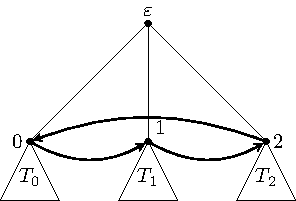
\includegraphics{figures/groupActions/tAction}
		\caption{action of $t$}
		\label{fig:action-t}
	\end{subfigure}
	\hfill
	\begin{subfigure}[b]{.48\linewidth}
		\centering
		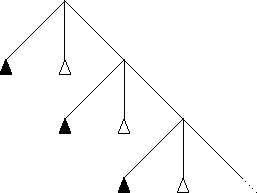
\includegraphics{figures/groupActions/zAction}
		\caption{action of $z$}
		\label{fig:action-z}
	\end{subfigure}

	\caption{Actions of $t$ and $z$ on $\mathcal{T}_3$}
	\label{fig:actions}
\end{figure}

In \cref{fig:action-t}, the first level of the tree is cyclically permuted, and the sub-trees $T_0$, $T_1$ and $T_2$ are fixed i.e.\ not permuted.
In \cref{fig:action-z}, the solid triangles, \tActionNotation, denote that an action of $t$ is taken on the associated sub-tree; and the hollow triangles, \idActionNotation, indicate that the associated sub-tree is fixed.

The \emph{Fabrykowski-Gupta group} is the group generated by the actions $t$ and $z$ as described earlier.

\begin{notation}
	Let $\mathbb{G} = \left\langle t, z \right\rangle$ denote the Fabrykowski-Gupta group
	\thmendmark
\end{notation}

Considering the geometric definition of the actions $t$ and $z$ given in \cref{fig:actions}, it can be seen that both $z^3$ and $t^3$ are equivalent to the identity as they fix $\mathcal{T}_3$.
Thus, elements of the Fabrykowski-Gupta group can be represented as alternating words of $t^{\pm 1}$ and $z^{\pm 1}$.
That is, words of the form
\begin{align*}
	\left(t^{\varepsilon_1}\right)\, z^{\delta_1}\,
	t^{\varepsilon_2}\, z^{\delta_2}\,
	\cdots
	t^{\varepsilon_n}\, z^{\delta_n}\,
	\left(t^{\varepsilon_{n+1}}\right)
\end{align*}
where each $\varepsilon_i, \delta_i \in \left\lbrace -1,1 \right\rbrace$, and the brackets, $(\cdot)$, indicate that the first and last $t^{\varepsilon_j}$ are optional.
This will be known as the \emph{alternating form} of words in the Fabrykowski-Gupta group.

Let $\Stab(1)$ be the subgroup of $\mathbb{G}$ that stabilises the first level of the tree $\mathcal{T}_3$, that is, the subgroup which doesn't permute the first level.
Notice that $\Stab(1)$ is generated by
\begin{align*}
	z_0 = z &= \recurDef{ t,1,z },
	&
	z_1 = z^t &= \recurDef{ z,t,1 },
	&
	z_2 = z^{t^{-1}} &= \recurDef{ 1,z,t }
\end{align*}
That is,
\[
\Stab(1) = \left\langle z_0, z_1, z_2 \right\rangle
\]
Thus, the Fabrykowski-Gupta group can be written as the semidirect product $\Stab(1) \rtimes \left\langle t \right\rangle$.
Therefore, every element of the Fabrykowski-Gupta group can be written in the form
\[
	\tau
	\,
	z_{c_1}^{\varepsilon_1}
	\,
	z_{c_2}^{\varepsilon_2}
	\cdots
	z_{c_n}^{\varepsilon_n}
	\quad
	\text{where}
	\quad
	c_i \in \left\lbrace 0,1,2 \right\rbrace,\ 
	\varepsilon_i \in \left\lbrace -1,1 \right\rbrace
	\text{ and }
	\tau \in \left\lbrace 1,t,t^{-1} \right\rbrace
\]
This will be known as the \emph{coset form} of words in the Fabrykowski-Gupta group.

\begin{remark}
	Neither the alternating form nor the coset form, as described earlier, represent elements in the Fabrykowski-Gupta group uniquely.
	Thus, neither of these forms are normal forms.
	The purpose and relevance of these two forms will become apparent in the following sections.
\end{remark}

\begin{note*}
	In subsequent sections of this chapter $X$ will denote the symmetric generating set of the Fabrykowski-Gupta group, that is, $X = \left\lbrace t^{\pm 1}, z^{\pm 1}\right\rbrace$.
\end{note*}

\section{Forms of Words}

This section will introduce some properties of the alternating and coset form, both of which ere defined previously in this chapter.

\begin{proposition}
	\label{prop:geodesics-in-alt-form}
	All geodesics of the Fabrykowski-Gupta group are in the alternating form.
\end{proposition}

\begin{proof} Let $w\in X^*$ be a word that is not in the alternating form.
	
	%Since $w$ is not in the alternating form, 
	Then either $w$ is not freely reduced or contains a subword $t^2$, $t^{-2}$, $z^2$ or $z^{-2}$;
	thus, a strictly shorter word $w^\prime$ can be obtained by either freely reducing $w$ or replacing one of the aforementioned subwords with $t^{-1}$, $t$, $z^{-1}$ or $z$, respectively. 
	
	Notice that the word $w^\prime$ and $w$  will correspond to the same group element.
	
	Thus, $w$ is not geodesic as there is a strictly shorter word $w^\prime$ that represents the same element.
\end{proof}

It is known that every element of the Fabrykowski-Gupta group can be represented by a word in the coset form.
However, the process of generating such a representation may not be as obvious.
The process of taking a word from the alternating form to the coset form is a simple rewrite procedure in which the letters of the word are read right-to-left; to understand the idea of this procedure, consider the following example.

\begin{example}
	Consider the word $t^{-1} z t z^{-1} t z$, in the alternating form, as follows.
	\begin{align*}
	  t^{-1} z t z^{-1} t z
	  &\mapsto t^{-1} z t z^{-1} t \left(z\right)
	   &&\left(z\text{ is already in the coset form}\right)
	   \\
	  &\mapsto t^{-1} z t^{-1} \left( t^{-1}  z^{-1} t\right) \left(z\right)
	   &&\left(\text{replaced a }t\text{ with }t^{-1}t^{-1}\right)
	   \\
	  &\mapsto t \left(t z t^{-1}\right) \left( t^{-1}  z^{-1} t\right) \left(z\right)
	   &&\left(\text{replaced a }t^{-1}\text{ with }tt\right)
	   \\
	  &\mapsto \left(t\right) \left(t z t^{-1}\right) \left( t^{-1}  z^{-1} t\right) \left(z\right)
	   &&\left(\text{only a }t\text{ remains}\right)
	   \\
	  &\mapsto t \, z_2 \, z_1^{-1} \, z_0
	   &&\left(\text{rewrite in the coset form}\right)
	\end{align*}
	Thus, it can be seen that $t^{-1} z t z^{-1} t z$ is equivalent to $t \, z_2 \, z_1^{-1} \, z_0$ in the coset form.
	\thmendmark
\end{example}

The previous example shows the idea of working from right-to-left over a word in the alternating form, matching conjugates of $z^{\pm 1}$ by replacing  $t$'s and $t^{-1}$ with $t^{-1}t^{-1}$ and $tt$, respectively, where necessary.
Considering this rewrite procedure, it can be seen that a word in the alternating form can be converted to the coset form in linear time with respect to word length of the input.
Thus, the following lemma results.

\begin{lemma}
	\label{lemma:coset-form-linear}
	A word $w \in X^\ast$ in the alternating form, can be converted to an equivalent word in the coset form in linear time with respect to the word length of $w$.
\end{lemma}

\begin{remark}
	\label{rmk:constantNumberZ}
	Notice that the previously described process does not replace or omit any $z$'s or $z^{-1}$'s.
	Thus, the word in the coset form obtained from the previously described procedure will have the same number of $z$'s and $z^{-1}$'s as the original word in the alternating form.
	\thmendmark
\end{remark}

The coset form is of interest as it allows for easy computation of word restrictions to the first level of the tree $\mathcal{T}_3$.
To compute these restrictions, the following maps will be defined.

\begin{definition}
	\label{def:phi-maps}
	Let the following maps $\phi_0$, $\phi_1$ and $\phi_2$  be defined as
	\begin{align*}
	\phi_0 &=
	\begin{cases}
	z_0 \mapsto t\\
	z_1 \mapsto 1\\
	z_2 \mapsto z
	\end{cases}
	&
	\phi_1 &=
	\begin{cases}
	z_0 \mapsto z\\
	z_1 \mapsto t\\
	z_2 \mapsto 1
	\end{cases}
	&
	\phi_2 &=
	\begin{cases}
	z_0 \mapsto 1\\
	z_1 \mapsto z\\
	z_2 \mapsto t
	\end{cases}
	\end{align*}
	where each $\phi_j$ maps $t \mapsto 1$ and preserved inverses.
	Now, define
	\[
	  \phi_j\left(
	    \tau
	    \,
	    z_{c_1}^{\varepsilon_1}
	    \,
	    z_{c_2}^{\varepsilon_2}
	    \cdots
	    z_{c_n}^{\varepsilon_n}
	  \right)
	  =
	  \phi_j\left(z_{c_1}^{\varepsilon_1}\right)
	  \phi_j\left(z_{c_2}^{\varepsilon_2}\right)
	  \cdots
	  \phi_j\left(z_{c_n}^{\varepsilon_n}\right)
	\]
	for each word $\tau \, z_{c_1}^{\varepsilon_1} \, z_{c_2}^{\varepsilon_2} \cdots z_{c_n}^{\varepsilon_n}$ in the coset form.
\end{definition}

\begin{proposition}
	\label{prop:word-restrictions}
	Given a word $w \in X^\ast$ in the coset form, the words $\phi_0(w)$, $\phi_1(w)$ and $\phi_2(w)$ are equivalent to the restrictions $\left. w \right\vert_0$, $\left. w \right\vert_1$ and $\left. w \right\vert_2$, respectively.
\end{proposition}

\begin{proof}
	This follows from the recursive definition of $z_0$, $z_1$ and $z_2$.
\end{proof}

\begin{proposition}
	\label{prop:phiLengthReduce}
	Given a word of length $n$, each of its restrictions to the first level, as computed by converting to the coset form then applying the appropriate map $\phi_j$, are of length at most $\left\lceil n / 2 \right\rceil$.
\end{proposition}

\begin{proof}
	This proof will first show the statement for words in the alternating form, and then extend it to all words in the language $X^\ast$.
	
	Let $w$ be a word in the alternating form of length $n$.\\
	Then, $w$ can contain at most $\left\lceil n/2 \right\rceil$ letters of the form $z^{\pm 1}$.
	
	Thus, by considering \cref{rmk:constantNumberZ}, it can be seen that the coset form of $w$, obtained by the earlier described procedure, can contain at most $\left\lceil n/2 \right\rceil$ letters of the form $z_j^{\pm 1}$ as each $z_j^{\pm 1}$ contains exactly one letter of the form $z^{\pm 1}$.
	
	Thus, by applying one of the maps $\phi_j$, a word of length at most $\left\lceil n/2 \right\rceil$ will be obtained.\\
	Thus, completing the proof for the case of words in the alternating form.
	
	To see that this result generalises to all words in the language $X^\ast$, let some word $w \in X^\ast$ of length $m$ be given.
	Then, by repeatedly performing free reduction and replacing occurances of $z^2$, $z^{-2}$, $t^{2}$ and $t^{-2}$ with $z^{-1}$, $z$, $t^{-1}$ and $t$, respectively, a word $w^\prime$ in the alternating form of length $n\leq m$ is obtained.
	
	By then applying the earlier argument of this proof to $w^\prime$, it can be seen that the first level restrictions of $w$ are of length at most $\left\lceil n / 2 \right\rceil \leq \left\lceil m / 2 \right\rceil$.
	Thus, completing the proof.
\end{proof}

A self-similar group $G$ that acts on a tree $B^\ast$ is said to be \emph{contracting} if there exists a finite set $\mathcal{N} \subset G$, called a \emph{nucleus}, such that for every element $g \in G$ there is an $N \in \mathbb{N}$ such that $\left. g \right\vert_b \in \mathcal{N}$ for every $b\in B^N$.
That is, the actions of $g$ on the $N$-th level of the tree $B^\ast$ are all in the set $\mathcal{N}$.
Notice that the aforementioned $N \in \mathbb{N}$ can be dependent on the element $g \in G$.

\begin{corollary}
	\label{cor:nucleus}
	Fabrykowski-Gupta is contracting with a nucleus of $\mathcal{N} = \left\lbrace 1, t^{\pm 1}, z^{\pm 1}\right\rbrace$.
\end{corollary}

\begin{proof}
	Let $w \in X^\ast$.
	Considering the previous proposition (\ref{prop:phiLengthReduce}), it can be seen that by an induction on the length of words, that there must exist some depth of the tree, $N$, for which all restrictions, $\left. w \right\vert_a$ with $a \in A^N$, to the $N$-th level are of word length $0$ or $1$.
	
	Thus, each of $\left. w \right\vert_a$ with $a\in A^N$ must be in the set $\mathcal{N}$ as this is the set of all words of length $0$ and $1$.
	
	Hence, Fabrykowski-Gupta is contracting with a nucleus of $\mathcal{N}$.
\end{proof}

From \cref{lemma:coset-form-linear}, it is known that a word can be converted from the alternating form to the coset form in linear time.
It is also true that any word in the language $X^\ast$ can be converted to the alternating form in linear time with respect to the word length of the input word.
To see this, let some word $w \in X^\ast$ in the alternating form be given.
Then, given some letter $a \in X$, the word $wa$ can be computed in the alternating form by considering the following two cases:
\begin{itemize}
	\item[(1)] If $w$ does not end in $a$ or $a^{-1}$ then simply concatenating the $a$ to the end of $w$ will result in a word in the alternating form;
	\item[(2)] If $w$ ends in $a$ or $a^{-1}$, then replace this letter with $a^{-1}$ or remove it, respectively.
\end{itemize}
Thus, appending a letter to a word in the alternating form, obtaining a result in the alternating form, can be done in constant time.

Hence, a word $w\in X^\ast$ of length $n = \left\vert w \right\vert$ can be converted to the alternating form by reading $w$ from left-to-right, appending its letters to a word $v$ in the alternating form to obtain a word in the alternating form.
Thus, if $v$ is initially the empty word, then after $n$ steps of a constant time procedure $v$ will contain an equivalent word in the alternating form.
Thus, the following results.

\begin{lemma}
	\label{lemma:alt-form-linear}
	A word $w \in X^\ast$ can be converted to an equivalent word in the alternating form in linear time with respect to the word length of $w$.
\end{lemma}

%\newpage
\section{Word Problem}
\label{sec:word-problem}

This section presents an efficient algorithm which solves the word problem for the Fabrykowski-Gupta group.
The details and complexity analysis of this algorithm will be provided as it is used by the brute force algorithm for generating geodesics, which will be described in the next chapter.
The purpose of this section is to show that the word problem, in the case of Fabrykowski-Gupta, is solvable in time $O(n \log n)$ with respect to the word length of input words.

The algorithm described in this section relies heavily on the maps $\phi_j$, as described in \cref{def:phi-maps,prop:word-restrictions}, to compute the restrictions of words.
The complexity of this algorithm will then be proven by the use of \cref{lemma:coset-form-linear,lemma:alt-form-linear,prop:phiLengthReduce,prop:word-restrictions,cor:nucleus}.

For the purpose of this section, unless otherwise specified, let $w \in X^\ast$ be some arbitrary word.

Considering that $w$ is equivalent to the identity of $\mathbb{G}$ if and only if its action fixes every node of the tree $\mathcal{T}_3$, then it can be seen that the word problem may be solved recursively as given in \cref{alg:word-problem} on the following page.

\begin{algorithm}[!ht]
	
	\Fn(){\WP{$w$}}{
		\KwData{an input word $w \in X^\ast$}
		\KwResult{true if and only if $w$ is equivalent to the identity}
		
		\BlankLine
		
		Convert $w$ to the alternating form\;
		\label{alg:word-problem:convert-to-alt}
		
		\BlankLine
		
		\If{$\left\vert w \right\vert = 0$}{
			\label{alg:word-problem:check-trivial}
			\Return{true}\tcc*{$w$ is the empty word}
		}
	
		\BlankLine
	
		\If{$\left\vert w \right\vert = 1$} {
			\label{alg:word-problem:check-generator}
			\Return{false}\tcc*{$w$ represents a generator}
		}
	
		\BlankLine
	
		\If{$w$ permutes the first level of $\mathcal{T}_3$}{
			\label{alg:word-problem:check-first-level}
			\Return{false}\tcc*{$w$ permutes the first level}
		}
	
		\BlankLine
	
		Convert $w$ to the coset form\;
		\label{alg:word-problem:convert-coset}
		
		\BlankLine
		
		\tcp{check the action on the left sub-tree}
		
		$v \gets \phi_0(w)$\;
		\label{alg:word-problem:left-rist}
		
		\If{\WP{$v$} $=$ false}{
			\label{alg:word-problem:left-rec}
			\Return{false}\tcc*{$w$ permutes the left sub-tree}
		}
	
		\BlankLine
	
	    \tcp{check the action on the middle sub-tree}
	    
		$v \gets \phi_1(w)$\;
		\label{alg:word-problem:middle-rist}
		
		\If{\WP{$v$} $=$ false}{
			\label{alg:word-problem:middle-rec}
			\Return{false}\tcc*{$w$ permutes the middle sub-tree}
		}
	
		\BlankLine
		
		\tcp{check the action on the right sub-tree}
	
		$v \gets \phi_2(w)$\;
		\label{alg:word-problem:right-rist}
		
		\If{\WP{$v$} $=$ false}{
			\label{alg:word-problem:right-rec}
			\Return{false}\tcc*{$w$ permutes the right sub-tree}
		}
	
		\BlankLine
	
		\Return{true}\tcc*{$w$ does not permute the first level or any sub-tree}
		\label{alg:word-problem:final-return}
	}
	
	\caption{Word Problem}
	\label{alg:word-problem}
\end{algorithm}

The idea of this algorithm is to first check that the action of $w$ fixes the first level of the tree $\mathcal{T}_3$, then recursively check that it fixed any of the sub-trees.
For this algorithm to be valid, it remains to be shown that it will terminate on any given input; to see this, consider the following theorem which shows an upper bound on the complexity of \cref{alg:word-problem}.

%\newpage
\begin{theorem}
	\label{thm:word-problem-complexity}
	\Cref{alg:word-problem} has a time complexity of $O(n\log n)$.
\end{theorem}

\begin{proof}

Let $n$ be the size of the input word i.e.\ $n = \left\vert w \right\vert$.

From \cref{prop:phiLengthReduce}, it can be seen that \cref{alg:word-problem} will only consider word restrictions down to a maximum depth of $\left\lceil \log_2 n \right\rceil$.
This is clear as at this depth, all word restrictions, as computed by appropriate applications of the maps $\phi_j$, will be of length $0$ or $1$, and thus \cref{alg:word-problem} will be able to return either `true' or `false' at, or before, this depth is reached.

Now, consider the complexity of each of the lines of the algorithm.
From \cref{lemma:alt-form-linear}, it is known that words can be converted to the alternating form in linear time, and thus \cref{alg:word-problem:convert-to-alt} will run in linear time; also and after this line $w$ can't increase in word length.
It is clear that a word's action on the first level of $\mathcal{T}_3$ can be checked in linear time (simply by considering the $t$'s and $t^{-1}$'s in $w$), and thus \cref{alg:word-problem:check-first-level} will run in linear time.
From \cref{lemma:alt-form-linear} it is known that words in the alternating form can be converted to the coset form in linear time, and thus \cref{alg:word-problem:left-rist,alg:word-problem:middle-rist,alg:word-problem:right-rist} will run in linear time.
All the remaining lines, except for the recursive calls on \cref{alg:word-problem:left-rec,alg:word-problem:middle-rec,alg:word-problem:right-rec}, will run in constant time.

Therefore, every line of \cref{alg:word-problem}, except for the recursive calls on \cref{alg:word-problem:left-rec,alg:word-problem:middle-rec,alg:word-problem:right-rec}, will run within linear time with respect to the size, $n$, of the input word.

Let $\#_z : X^\ast \to \mathbb{N}$ count the number of $z$'s and $z^{-1}$'s in a word.
For example, $\#_z\left(tztz^{-1}t^{-1}\right) = 2$.

In the remainder of this proof, let $\left. w \right\vert_a$ denote the word restriction of $w$ to $a$ as calculated by an appropriate sequence of applications of the maps $\phi_j$.

Now, considering the maps $\phi_j$, as given in \cref{def:phi-maps}, it can be seen that the following inequality holds for $w$ in the alternating form
\[
\#_z(w) \geq
\#_z\left(\left. w \right\vert_0 \right) +
\#_z\left(\left. w \right\vert_1 \right) +
\#_z\left(\left. w \right\vert_2 \right)
\]
Hence by induction, for any depth, $m$, of the tree $\mathcal{T}_3$ then,
\[
\#_z(w) \geq
\sum_{a \in A^m}
\#_z\left(\left. w \right\vert_a \right)
\]
where $m \in \mathbb{N}$ is a depth of the tree $\mathcal{T}_3$.

Now considering again the maps $\phi_j$, and the recursive definition of $z$ as $\recurDef{t,1,z}$, it can be seen that the total word length of the restrictions to the $m$-th level of $\mathcal{T}_3$ can be no more than two times the total number of $z$'s and $z^{-1}$'s in the word restrictions on the $(m-1)$-th level, that is,
\[
  \sum_{a \in A^{m}}
  n_a
  \leq
  2
  \sum_{a \in A^{m-1}} \#_z\left(\left. w \right\vert_a \right)
\]
where $n_a$ is the word length of the restriction $\left. w \right\vert_a$.
Thus, for $m > 0$,
\[
  \sum_{a \in A^{m}}
  n_a
  \leq
  2
  \cdot
  \#_z(w)
\]
Further, with $w$ in the alternating form, it follows that $\#_z(w)$ can be no more than $\left\lceil n/2 \right\rceil$ where $n$ is the word length of $w$.
Thus,
\[
  \sum_{a \in A^{m}}
  n_a
  \leq
  2
  \left\lceil n/2 \right\rceil
  \ \ 
  \text{for all }
  m > 0
  \text{, and thus,}
  \ \ 
  \sum_{a \in A^{m}}
  n_a
  \leq
  n+1
  \ \ 
  \text{for all levels }m \in \mathbb{N}\text{ of }\mathcal{T}_3.
\]
Thus, for each level $m \in \mathbb{N}$ of the tree $\mathcal{T}_3$, a linear time algorithm (i.e.\ everything except the recursive calls of \cref{alg:word-problem:left-rec,alg:word-problem:middle-rec,alg:word-problem:right-rec}) will be run $\ell$ times on inputs of word length $n_1$, $n_2$, \ldots, $n_\ell$, respectively, where $n_1 + n_2 + \cdots + n_\ell \leq n+1$.
Notice that instances where the algorithm is run with input of word length zero can be ignored as their run-times are constant and can be considered a part of the run-time of their respective callers.

Thus, \cref{alg:word-problem} is composed of no more than $\left\lceil \log_2 n \right\rceil$ instances (one for each level) of an algorithm of complexity $O(n)$.
Hence, the complexity of \cref{alg:word-problem} is $ O(\left\lceil \log_2 n \right\rceil n)$.

Therefore, the complexity of \cref{alg:word-problem} is $O(n \log n)$ as required.
\end{proof}

%\newpage
\section{Signatures}

This section will introduce three functions known which will be known as the signatures.
These functions were originally designed with the intention of improving the run-time of the brute force geodesic generating algorithm, which will be presented in \cref{sec:growth-functions}, by a constant factor.
However, these functions later became important when defining an algorithm, which will be presented in the next section, to compare words of the Fabrykowski-Gupta group.

This section will begin by defining the functions $\sig_t,\sig_z : X^\ast \to \left\lbrace 0, 1, 2 \right\rbrace$ which will be known as the $t$ and $z$ signatures, respectively.
These signatures will then be shown to be homomorphisms when considered as maps $\mathbb{G} \to (\mathbb{Z}/3\mathbb{Z}, +)$, and thus for any two words $w,v \in X^\ast$ with $w =_\mathbb{G} v$, it follows that $\sig_t(w) = \sig_t(v)$ and $\sig_z(w) = \sig_z(v)$.

Let some $w \in X^\ast$ be chosen, then the signatures $\sig_t(w)$ and $\sig_z(w)$ are defined as follows.

\begin{definition}
	\label{def:t-signature}
	The \emph{$t$-signature} of $w$, denoted $\sig_t(w)$, is the sum of powers of $t$ in $w$ modulo 3.
\end{definition}

\begin{example}
	To understand the $t$-signature, consider the following examples.
	\begin{align*}
	  \sig_t\left( z^n \right)         &= 0,             &
	  \sig_t\left( t^nzt^{-m} \right)         &\equiv (n-m) \mod 3, &
	  \sig_t\left( t^{-1}z t^2 \right) &= 1
	\end{align*}
\end{example}

\begin{definition}
	\label{def:z-signature}
	The \emph{$z$-signature} of $w$, denoted $\sig_z(w)$, is the sum of powers of $z$ in $w$ modulo 3.
\end{definition}

\begin{example}
	To understand the $z$-signature, consider the following examples.
	\begin{align*}
	\sig_z\left( z^n \right)     &\equiv n \mod 3, &
	\sig_z\left( t^n \right)     &= 0,             &
	\sig_z\left( z t z^{-1}\right) &= 0
	\end{align*}
	\thmendmark
\end{example}

Notice that the signature $\sig_t(w)$ indicates how the word $w$ permutes the first level of the tree $\mathcal{T}_3$, that is, $\sig_t(w)$ is; $0$ if $w$ fixes the first level; $1$ if $w$ performs $t$ to the first level; and $2$ if $w$ performs $t^{-1}$ to the first level.
Then, since words which represent the same group element permute the first level in the same way, it follows that two such words have the same $t$-signature.
Thus, the $t$-signatures can be viewed as a map from $\mathbb{G}$ to the group $\left\langle t \, \middle\vert \, t^3 \right\rangle \cong (\mathbb{Z}/3\mathbb{Z},+)$.
Further, it can be seen that this map is in fact a homomorphism by considering the way in which words are composed.
Thus, the following proposition follows.

\begin{proposition}
	The $t$-signature function can be seen to be a homomorphism when viewed as a function which maps $\mathbb{G} \to (\mathbb{Z}/3\mathbb{Z},+)$.
	\thmendmark
\end{proposition}

It will now be shown that the $z$-signature function is also a homomorphism when taken to be a map $\mathbb{G} \to (\mathbb{Z}/3\mathbb{Z},+)$.
To do this, it will first be shown that $\sig_z(w) = 0$ whenever $w$ is equivalent to the identity. Now, considering the definition of the maps $\phi_j$ in \cref{def:phi-maps}, and \cref{prop:word-restrictions}, it can be seen that
\[
  \sig_z(w)
  \equiv
  \sig_t(\left. w \right\vert_0) +
  \sig_t(\left. w \right\vert_1) +
  \sig_t(\left. w \right\vert_2)
  \pmod{3}
\]
where each $\left. w \right\vert_j$ is calculated by the corresponding $\phi_j$ map.
Then, since $w$ is equivalent to the identity, it follows that each of the $\sig_t(\left. w \right\vert_j)$ it the above must be zero, and hence, $\sig_z(w) \equiv 0 \pmod{3}$.
Therefore, $\sig_z$ maps every word which is equivalent to the identity to zero as required.

Now, considering the way in which word inverses are calculated and concatenation of words, it can be seen that $\sig_z(w) + \sig_z(w^{-1}) = 0$ and $\sig_z(wv) = \sig_z(w) + \sig_z(v) \pmod{3}$ for all $w,v\in X^\ast$.
Let $w,v\in X^\ast$ be words such that $w =_\mathbb{G} v$, then
\[
  0 = \sig_z(w v ^{-1}) = \sig_z(w) - \sig_z(v)
\]
and thus, $\sig_z(w) = \sig_z(v)$.
Thus, $\sig_z$ can be viewed as a map from $\mathbb{G}$ to $(\mathbb{Z}/3\mathbb{Z},+)$ that preserves the group structure.
Thus, the following proposition results.

\begin{proposition}
	The $z$-signature function can be seen to be a homomorphism when viewed as a function which maps $\mathbb{G} \to (\mathbb{Z}/3\mathbb{Z},+)$.
	\thmendmark
\end{proposition}

For the purpose of convenience, the following additional signature will be defined.

\begin{definition}
	\label{def:full-signature}
	The \emph{full-signature} of $w$, denoted $\sig(w)$, is defined as
	\[
	  \sig(w) \coloneqq 3\cdot\sig_z(w) + \sig_t(w)
	  \in \left\{ 0,1,2,\ldots, 8 \right\}
	\]
	Thus, $\sig(w)$ can be viewed as a homomorphism $\mathbb{G} \to (\mathbb{Z}/3\mathbb{Z},+)^2$,
	where the elements of the form $(i,j) \in (\mathbb{Z}/3\mathbb{Z},+)^2$ are represented by the corresponding integers $(3\cdot i) + j$.
	Further, it can be seen that both $\sig_t(w)$ and $\sig_z(w)$ are recoverable from $\sig(w)$.
\end{definition}

\begin{remark}
	The full-signature of a word is represented as an integer in $\left\lbrace 0, 1, 2,\ldots, 8 \right\rbrace$, rather than a tuple of the form $\left\lbrace 0,1,2 \right\rbrace^2$, as this form becomes convenient when defining the word comparison algorithm of the next section.
\end{remark}

\begin{remark}
	Elements of the nucleus, $\mathcal{N} = \left\lbrace 1, t^{\pm 1}, z^{\pm 1} \right\rbrace$, are each assigned a different value by $\sig$, and thus elements of the nucleus are recoverable from their corresponding full signatures.
\end{remark}

\section{Comparing Words}
\label{sec:comparing-words}

This section will describe an algorithm that can compare any two words in the Fabrykowski-Gupta group in the sense that, given two words $w,v\in X^\ast$, then exactly one of $w < v$, $v < w$ or $w =_\mathbb{G} v$ will be true where $<$ is taken with respect to the comparison.
Further, this comparison algorithm will satisfy transitivity in the sense that, given some $u,v,w\in X^\ast$ such that $u < v$ and $v < w$, it follows that $u < w$.
This comparison algorithm then makes it possible to sort a list of words in the language $X^\ast$ with the use of a comparison-based sort algorithm.
This fact will be used in \cref{sec:sortingMethod} where it will be shown that the geodesics of the Fabrykowski-Gupta group may be generated efficiently by a modified sort algorithm.

The comparison algorithm described in this section is based on a variation of what are known as portraits.
A \emph{portrait} is a finite rooted tree where each node is decorated to shows how its corresponding sub-tree is permuted, and the leaves are decorated with an element of the group's nucleus.
For example, a portrait of the word $tztztztztz^{-1}t$ is given as in \cref{fig:tztztztztZtPortrait}.

\begin{figure}[!ht]
	\centering
	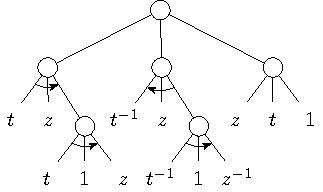
\includegraphics[width=.4\linewidth]{figures/portraits/tztztztztZtPortrait}

	\caption{A portrait of the word $tztztztztz^{-1}t$.}
	\label{fig:tztztztztZtPortrait}
\end{figure}

Notice that in \cref{fig:tztztztztZtPortrait} as above, an arrow from left-to-right indicates an action of $t$, an arrow from right-to-left indicated an action of $t^{-1}$, and the absence of an arrow indicated that the associated sub-tree is not cyclically permuted.
The action of a portrait should be read such that the actions of the leaves being applied first, followed by the arrows in a bottom-up order; the idea being that the action of the portrait is equivalent to the action of the corresponding group element.

Notice that any portrait can be written such that it's leaves are on the same level.
For example, \cref{fig:port2} shows an equivalent portrait for $tztztztztz^{-1}t$ (compare this with the previous portrait).

\begin{figure}[!ht]
\begin{center}
	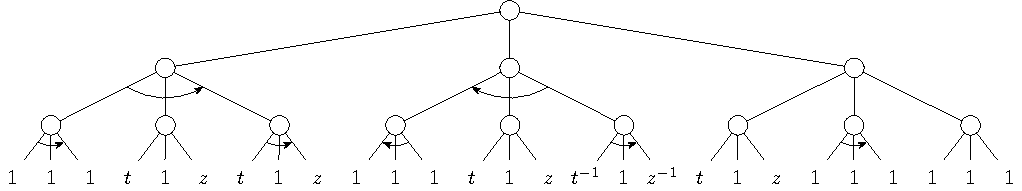
\includegraphics[width=\linewidth]{figures/portraits/tztztztztZtPortraitFull}
\end{center}
	\caption{A depth three portrait for $tztztztztz^{-1}t$.}
	\label{fig:port2}
\end{figure}

\begin{remark}
	Note that it is possible to define (finite) portraits in any contracting group.
	\thmendmark
\end{remark}

As was mentioned previously, the algorithm of this section is based on a modified version of these portraits.
In this modified version, which will be known as the \emph{signature portrait}, the finite trees are instead decorated with word signatures as in \cref{def:full-signature}.
For example, the words $z^{-1}tztzt$ and $z^{-1}tzt^{-1}zt^{-1}ztz^{-1}$ have the  (regular) portraits shown in \cref{fig:port3}. % respectively.

\begin{figure}[!ht]
	\centering
	
	\hfill
	\begin{subfigure}{.45\linewidth}
		\centering
		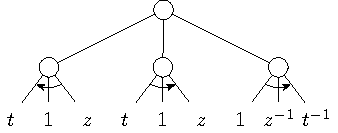
\includegraphics[width=\linewidth]{figures/portraits/ZtztztPortrait}
	\end{subfigure}
	\hfill
	\begin{subfigure}{.45\linewidth}
		\centering
		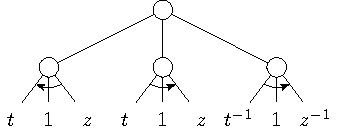
\includegraphics[width=\linewidth]{figures/portraits/ZtzTzTztZPortrait}
	\end{subfigure}
	\hfill

	\caption{(Regular) portraits for $z^{-1}tztzt$ and $z^{-1}tzt^{-1}zt^{-1}ztz^{-1}$, respectively.}
	\label{fig:port3}
\end{figure}

Now signature portraits of words $z^{-1}tztzt$ and $z^{-1}tzt^{-1}zt^{-1}ztz^{-1}$ are given in \cref{fig:port4}.

\begin{figure}[!ht]
\begin{center}
	
	\hfill
	\begin{minipage}{.45\linewidth}
		\centering
		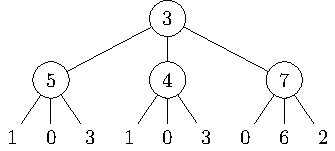
\includegraphics[width=\linewidth]{figures/portraits/ZtztztSigPortrait}
	\end{minipage}
	\hfill
	\begin{minipage}{.45\linewidth}
		\centering
		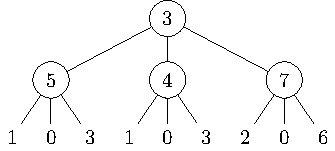
\includegraphics[width=\linewidth]{figures/portraits/ZtzTzTztZSigPortrait}
	\end{minipage}
	\hfill
	
\end{center}
\caption{Signature portraits for $z^{-1}tztzt$ and $z^{-1}tzt^{-1}zt^{-1}ztz^{-1}$, respectively}
	\label{fig:port4}
\end{figure}



Notice that in the signature portrait, the leaves must correspond to a node of the tree in which the word performs an action from the nucleus.
Also, the numbers on the leaves and nodes correspond to the value that `$\sig$' (see \cref{def:full-signature}) assigns to the corresponding word restrictions.

\begin{remark}
	A portrait is recoverable from each signature portrait; the elements on the leaves are recoverable as `$\sig$' assigns a different value to each element in the nucleus $\mathcal{N} = \left\lbrace 1,t^{\pm 1}, z^{\pm 1}\right\rbrace$; the arrows on the nodes are recoverable from the value of $\sig_t$ which is itself recoverable from  $\sig$.
	
	Hence, elements of the Fabrykowski-Gupta can be represented faithfully by signature portraits.
	\thmendmark
\end{remark}

Given two words $w,v \in X^\ast$, the idea of the comparison algorithm is to construct signature portraits for $w$ and $v$ of the same depths and to compare the trees in a depth-first order.
For example, the two signature portraits given earlier can be viewed as tuples $\mathbf{x} = (3,5,1,0,3,4,1,0,3,7,0,6,2)$ and $\mathbf{y} = (3,5,1,0,3,4,1,0,3,7,2,0,6)$, respectively, when the values are read in a depth-first order.
Notice that these tuples match in the first $10$ entries, but in the $11$-th entry $0 = \mathbf{x}_{11} < \mathbf{y}_{11} = 2$.
Hence, it is said that $\mathbf{x} < \mathbf{y}$, and thus $z^{-1}tztzt< z^{-1}tzt^{-1}zt^{-1}ztz^{-1}$ under the comparison.

Notice that such a comparison is transitive by the transitivity of integer comparison, and that the required trichotomy holds as exactly one of $\mathbf{x} < \mathbf{y}$,  $\mathbf{y}< \mathbf{x}$ or  $\mathbf{x} =  \mathbf{y}$ will hold, where $\mathbf{x} =  \mathbf{y}$ holds if and only if the two signature portraits are identical and thus represent the same element.

Building the entire signature portraits of the two elements, as described earlier, may produce redundant or unused information.
The algorithm, which is described on the next page, will avoid this problem by recursively generating only the sections of the tree that would be required under this procedure.
For a complete understanding of the comparison algorithm the reader should study the pseudocode provided in \cref{alg:compare-words} on the following page.

%\newpage

\begin{algorithm}[!ht]
	
	\Fn(){\COMP{$w, v$}}{
		\KwData{input words $w,v \in X^\ast$}
		\KwResult{returns $0$ if $w =_\mathbb{G} v$; $-1$ if $w < v$; or $1$ if $w > v$}
		
		\BlankLine
		
		\tcp{Generate the signatures of the input words}
		$s_1 \gets \sig(w)$\;
		$s_2 \gets \sig(v)$\;
		
		\BlankLine
		\BlankLine
		
		\tcp{Check if the two signatures are different}
		
		\BlankLine
		
		\If{$s_1 < s_2$}{
			\Return{$-1$}\tcc*{by the ordering, $w_1 < w_2$}
		}
		\BlankLine
		\If{$s_1 > s_2$}{
			\Return{$1$}\tcc*{by the ordering, $w_1 > w_2$}
		}
	
		\BlankLine
		\BlankLine
		
		\tcp{The signatures are the same\\Thus, check if the nucleus has been reached}
		
		\If{
			$\left\vert w \right\vert \leq 1$
			 and
			$\left\vert v \right\vert \leq 1$
		}{
			\Return{$0$}\tcc*{both $w$ and $v$ are in the nucleus, hence, $w =_\mathbb{G} v$}
		}
	
		\BlankLine
	
		\tcp{The lines in the `for' loop require $w$ and $v$ to be in the coset form}
		Convert $w$ and $v$ to the coset form\;
	
		\BlankLine
		\tcp{It is still possible that the words $w$ and $v$ represent different actions\\
		Thus, check the sub-trees recursively as follows}
	
		\BlankLine
		
		\For{$j$ from $0$ to $2$}{
			\tcp{Notice that $j \in \{0,1,2\}$ corresponds to the sub-trees}
			
			\BlankLine
			
			\tcp{Compute the restrictions to the $j$-th sub-tree}
			
			\BlankLine
			
			$w^\prime \gets \phi_j(w)$\;
			$v^\prime \gets \phi_j(v)$\;
			
			\BlankLine
			
			Convert $w^\prime$ to the alternating form\;
			Convert $v^\prime$ to the alternating form\;
			
			\BlankLine
			
			\tcp{Compare the sub-trees}
			
			\BlankLine
			
			$c \gets$ \COMP{$w^\prime$, $v^\prime$}\;
			
			\BlankLine
			
			\tcp{Check if the sub-trees were found not to be equal}
			
			\BlankLine
			\If{$c \neq 0$}{
				\Return{$c$}\tcc*{$c$ is the desired comparison with respect to the ordering}
			}
	
		}
	
		\BlankLine
	
		\tcp{All sub-trees have the same signature}
		
		\BlankLine
		
		\Return{$0$}\;
		
	}
	
	\caption{Compare Word}
	\label{alg:compare-words}
\end{algorithm}

\begin{theorem}
	\label{thm:comparison-algorithm-complexity}
	The time complexity of \cref{alg:compare-words} is $O(n\log n)$ where $n$ is the word length of the largest input, that is, $n = \max\left\{ \left\vert w\right\vert, \left\vert v \right\vert \right\}$ where $w$ and $v$ are the words being compared.
\end{theorem}

\begin{proof}
	Comparing \cref{alg:compare-words} to \cref{alg:word-problem}, it can be seen that the computations involved are very similar; except in \cref{alg:compare-words}, in some sense, they are performed twice.
	Thus, considering the proof of \cref{thm:word-problem-complexity}, it can be seen that the complexity of this algorithm is $O(\max\left\{
		\left\vert w \right\vert \log \left\vert w \right\vert,
		\left\vert v \right\vert \log \left\vert v \right\vert
	\right\})$
	where $w$ and $v$ are the two input words to the algorithm.
	
	Therefore, the complexity of the algorithm is $O(n\log n)$ as required.
\end{proof}
